\documentclass[12pt,a4paper]{article}

% ==============================================================================
% PAQUETES DE CONFIGURACIÓN Y ESTILO
% ==============================================================================
\usepackage[utf8]{inputenc}
\usepackage[T1]{fontenc}
\usepackage{lmodern}
\usepackage[spanish,es-tabla,es-nodecimaldot]{babel}
\usepackage[margin=2.5cm,top=3cm,bottom=3cm,headheight=15pt]{geometry}
\usepackage{graphicx}
\usepackage{float}
\usepackage{booktabs}
\usepackage{amsmath,amssymb}
\usepackage{xcolor}
\usepackage{fancyhdr}
\usepackage{titlesec}
\usepackage{setspace}
\usepackage{tabularx}
\usepackage{caption}
\usepackage{subcaption}
\usepackage{enumitem}
\usepackage{microtype}
\usepackage[colorlinks=true,linkcolor=teal!80!black,urlcolor=blue!70!black,citecolor=teal!70!black]{hyperref}

% Configuración de ruta de imágenes
\graphicspath{{figuras/}}

% Paleta de colores institucionales y de diseño
\definecolor{TealPrimary}{HTML}{00696D}
\definecolor{TealDark}{HTML}{004D40}
\definecolor{SlateDark}{HTML}{0F172A}
\definecolor{SlateLight}{HTML}{F8FAFC}
\definecolor{AccentGreen}{HTML}{047857}
\definecolor{AccentAmber}{HTML}{D97706}
\definecolor{AccentRed}{HTML}{B91C1C}

% Configuración de encabezados y pies de página
\pagestyle{fancy}
\fancyhf{}
\fancyhead[L]{\small \textcolor{gray}{\textit{SoundscapeMapper --- Aplicaciones Móviles II}}}
\fancyhead[R]{\small \textcolor{gray}{\textit{Proyecto Final}}}
\fancyfoot[C]{\thepage}
\renewcommand{\headrulewidth}{0.4pt}
\renewcommand{\footrulewidth}{0.4pt}

% Formato de títulos
\titleformat{\section}
  {\normalfont\Large\bfseries\color{TealDark}}{\thesection.}{0.8em}{}
\titleformat{\subsection}
  {\normalfont\large\bfseries\color{TealPrimary}}{\thesubsection.}{0.6em}{}
\titleformat{\subsubsection}
  {\normalfont\normalsize\bfseries\color{SlateDark}}{\thesubsubsection.}{0.5em}{}

\setstretch{1.15}
\setlength{\parskip}{6pt}
\setlength{\parindent}{0pt}

% ==============================================================================
% INICIO DEL DOCUMENTO
% ==============================================================================
\begin{document}

% ------------------------------------------------------------------------------
% PORTADA
% ------------------------------------------------------------------------------
\begin{titlepage}
    \centering
    \vspace*{0.5cm}
    
    {\scshape\LARGE Universidad Tecnológica / Politécnica \par}
    \vspace{0.3cm}
    {\scshape\large División de Tecnologías de la Información y Comunicación \par}
    {\large Ingeniería en Desarrollo y Gestión de Software \par}
    
    \vspace{1.5cm}
    \rule{\linewidth}{1.5pt} \\[0.4cm]
    {\huge \bfseries \color{TealDark} SoundscapeMapper \par}
    \vspace{0.3cm}
    {\Large \textbf{Sistema Móvil Multisensor de Monitoreo Acústico, Confort Lumínico y Geolocalización Urbana Basado en Directrices de la OMS} \par}
    \rule{\linewidth}{1.5pt}
    
    \vspace{1.5cm}
    
    \begin{minipage}[t]{0.48\textwidth}
        \textbf{Asignatura:}\\
        Aplicaciones Móviles II\\[0.4cm]
        \textbf{Profesor:}\\
        Ing. / Mtro. Miguel Ángel Montoya Cerro\\[0.4cm]
        \textbf{Cuatrimestre y Grupo:}\\
        09\_01
    \end{minipage}
    \hfill
    \begin{minipage}[t]{0.48\textwidth}
        \begin{flushright}
            \textbf{Integrantes del Equipo:}\\
            Cristopher López Suárez\\
            Román Méndez Meneses\\
            Jovanny Hernández Hernández\\[0.4cm]
            \textbf{Tipo de Entrega:}\\
            Documentación Técnica de Proyecto Final
        \end{flushright}
    \end{minipage}
    
    \vfill
    {\large \textbf{Pachuca, Hidalgo, México}}\\[0.2cm]
    {\large Agosto 2026}
\end{titlepage}

% ------------------------------------------------------------------------------
% ÍNDICES
% ------------------------------------------------------------------------------
\newpage
\tableofcontents

\newpage
\listoffigures

\newpage

% ------------------------------------------------------------------------------
% RESUMEN
% ------------------------------------------------------------------------------
\section{Resumen}

El presente documento técnico detalla el diseño, arquitectura de software, desarrollo, pruebas y resultados de \textbf{SoundscapeMapper}, una aplicación móvil nativa para el sistema operativo Android orientada al monitoreo ambiental y a la preservación de la salud auditiva y el confort urbano. Desarrollada bajo el paradigma declarativo de \textbf{Jetpack Compose} en lenguaje \textbf{Kotlin}, la plataforma integra en tiempo real la captura del micrófono ($dB_{SPL}$), el sensor de iluminancia ambiental (Lux) y el sistema de geolocalización satelital (\textit{Fused Location Provider}). 

Los datos recabados se evalúan bajo las normativas de confort y umbrales de riesgo de la Organización Mundial de la Salud (OMS) y se gestionan de manera local y persistente mediante una base de datos relacional orientada a objetos con \textbf{Room (SQLite)}. Asimismo, se incorpora cartografía digital mediante \textit{OpenStreetMap} para la georreferenciación de estancias y refugios sonoros en la zona metropolitana de Pachuca, un servicio en segundo plano (\textit{Foreground Service}) con notificaciones y vibración háptica ante sobreexposiciones, y un motor analítico con gráficas dinámicas de barras animadas.

\vspace{0.3cm}
\textbf{Palabras clave:} Jetpack Compose, Room Database, Contaminación Acústica, Confort Lumínico, Organización Mundial de la Salud, Sensor de Luz, Micrófono, GPS, Foreground Service.

% ------------------------------------------------------------------------------
% INTRODUCCIÓN
% ------------------------------------------------------------------------------
\section{Introducción}

En los entornos urbanos contemporáneos, la contaminación acústica representa una de las problemáticas de salud pública más críticas y menos atendidas. De acuerdo con informes epidemiológicos de la Organización Mundial de la Salud (OMS), la exposición sostenida a niveles de ruido ambiental superiores a los 70--80 dB ocasiona efectos auditivos directos (hipoacusia inducida por ruido, acúfenos o tinnitus) e impactos extrauditivos de gravedad comprobada, tales como trastornos del sueño, elevación de la presión arterial, aumento del estrés crónico y deterioro de la concentración cognitiva.

De forma complementaria, el confort visual en espacios cerrados y abiertos se encuentra condicionado por la iluminancia ambiental: condiciones por debajo de los 100 lux o por encima de los 2500 lux inducen fatiga ocular, cefaleas y bajo rendimiento escolar y laboral.

A pesar del impacto de estas variables en la calidad de vida de los ciudadanos, existe un vacío tecnológico significativo: la población carece de herramientas móviles accesibles que permitan registrar, mapear y evaluar de manera integral las condiciones acústicas y lumínicas de su entorno cotidiano.

Ante este reto surge \textbf{SoundscapeMapper}, una solución tecnológica integral que convierte el dispositivo móvil en una estación portátil de monitoreo multisensorial, permitiendo diagnosticar la calidad del hábitat sonoro, identificar refugios de silencio y promover hábitos de higiene auditiva.

% ------------------------------------------------------------------------------
% OBJETIVOS
% ------------------------------------------------------------------------------
\section{Objetivo General}

Desarrollar una aplicación móvil nativa para el sistema operativo Android utilizando el lenguaje Kotlin, Jetpack Compose y la base de datos Room, que integre múltiples sensores físicos del dispositivo (micrófono, fotómetro de luz ambiental y geolocalización satelital GPS) para monitorizar, registrar, clasificar y cartografiar niveles de ruido e iluminancia conforme a los estándares de la Organización Mundial de la Salud (OMS), contribuyendo a la salud auditiva y al confort urbano.

\section{Objetivos Específicos}

\begin{enumerate}[label=\textbf{\arabic*.}]
    \item \textbf{Implementar el procesamiento digital de señales acústicas en tiempo real}: Capturar el flujo de audio mediante la API \texttt{AudioRecord}, calculando el valor eficaz de presión sonora (RMS) y su conversión a decibelios ponderados ($dB_{SPL}$) clasificados según la escala de la OMS.
    \item \textbf{Integrar sensores ambientales complementarios}: Adquirir lecturas en tiempo real del sensor de iluminancia física (\texttt{Sensor.TYPE\_LIGHT}) en lux y del proveedor de ubicación satelital (\texttt{FusedLocationProviderClient}) para georreferenciar cada muestra.
    \item \textbf{Construir un esquema de persistencia local robusto}: Implementar una base de datos relacional con **Room Database** con operaciones CRUD completas y consultas analíticas de agregación (\texttt{AVG}, \texttt{MAX}, \texttt{COUNT}).
    \item \textbf{Diseñar una interfaz declarativa interactiva y accesible}: Construir vistas mediante Jetpack Compose y Material Design 3 con diseño de alto contraste y retroalimentación háptica.
    \item \textbf{Desarrollar un servicio en segundo plano de alerta temprana}: Diseñar un \texttt{ForegroundService} que supervise continuamente el umbral auditivo configurado por el usuario, emitiendo notificaciones y patrones de vibración cuando se detecte riesgo auditivo.
    \item \textbf{Validar el funcionamiento global}: Aplicar pruebas unitarias sobre algoritmos espaciales (Haversine) y verificar el desempeño concurrente mediante corrutinas de Kotlin.
\end{enumerate}

% ------------------------------------------------------------------------------
% PLANTEAMIENTO DEL PROBLEMA
% ------------------------------------------------------------------------------
\section{Planteamiento del Problema}

En zonas urbanas de rápido crecimiento demográfico y comercial, como la ciudad de Pachuca de Soto, Hidalgo, los estudiantes y trabajadores están sometidos a fuentes acústicas desreguladas: transporte colectivo ruidoso, congestión vehicular en avenidas principales, obras de construcción y establecimientos comerciales con perifoneo no controlado.

Las principales deficiencias detectadas son:
\begin{itemize}[leftmargin=*]
    \item \textbf{Invisibilidad de la dosis sonora diaria}: El usuario desconoce la acumulación de energía acústica recibida a lo largo de su jornada, superando inadvertidamente los límites seguros recomendados por la OMS.
    \item \textbf{Dificultad para localizar espacios de confort}: Carencia de un mapa interactivo que geolocalice cafeterías, bibliotecas o parques tranquilos (<65 dB) y adecuadamente iluminados (300--750 lux).
    \item \textbf{Falta de aplicaciones integrales e independientes}: Las soluciones existentes en las tiendas de aplicaciones se limitan a sonómetros simples sin almacenamiento local estructurado, sin evaluación multisensorial cruzada y sin enfoque educativo.
\end{itemize}

% ------------------------------------------------------------------------------
% ESTADO DEL ARTE
% ------------------------------------------------------------------------------
\section{Estado del Arte}

Se realizó un análisis comparativo de las aplicaciones comerciales y académicas más representativas disponibles en la actualidad:

\begin{table}[H]
\centering
\small
\caption{Comparativa técnica entre soluciones existentes y SoundscapeMapper.}
\begin{tabularx}{\textwidth}{lccccc}
\toprule
\textbf{Solución} & \textbf{Sensores} & \textbf{Base de Datos} & \textbf{Georreferenciación} & \textbf{Luz (Lux)} & \textbf{Enfoque OMS} \\
\midrule
Sound Meter & Micrófono & No & No & No & No \\
Decibel X & Micrófono & Parcial (pago) & Parcial & No & Parcial \\
Lux Light Meter & Luz & No & No & Sí (aislado) & No \\
NIOSH Sound Level & Micrófono & Export CSV & No & No & Sí (Laboral) \\
\textbf{SoundscapeMapper} & \textbf{Mic + Luz + GPS} & \textbf{Room (SQLite)} & \textbf{Sí (OSM Nativo)} & \textbf{Sí} & \textbf{Sí (Integral)} \\
\bottomrule
\end{tabularx}
\end{table}

\textbf{Diferenciales clave de SoundscapeMapper:}
\begin{itemize}[leftmargin=*]
    \item \textbf{Procesamiento en el borde (\textit{Edge Computing})}: Las muestras acústicas se procesan de forma matemática local sin almacenar ni transmitir grabaciones de voz, garantizando privacidad absoluta.
    \item \textbf{Persistencia relacional enriquecida}: Almacenamiento continuo con Room que permite consultas dinámicas de promedios, picos máximos históricos y filtros por estado de iluminación.
    \item \textbf{Algoritmo espacial Haversine}: Cálculo automático de distancias a refugios sonoros preestablecidos (ej. Biblioteca Central Ricardo Garibay, Parque Ben Gurión).
\end{itemize}

% ------------------------------------------------------------------------------
% DESARROLLO DEL PROYECTO
% ------------------------------------------------------------------------------
\section{Desarrollo del Proyecto}

\subsection{Diseño de la Aplicación y Arquitectura}

El proyecto se estructuró bajo el patrón de arquitectura recomendado por Google: **MVVM (Model--View--ViewModel)**, desacoplando completamente la lógica de negocio, la capa de sensores y la capa de presentación declarativa:

\begin{itemize}[leftmargin=*]
    \item \textbf{Capa de Presentación (UI)}: Vistas declarativas en Jetpack Compose (\texttt{SplashScreen}, \texttt{HoyScreen}, \texttt{MapaScreen}, \texttt{RegistroScreen}, \texttt{AnalisisScreen}, \texttt{YoScreen}).
    \item \textbf{Capa de Controladores (ViewModels)}: \texttt{RegistroViewModel}, \texttt{SensorStateHolder} que publican flujos de estado inmutables (\texttt{StateFlow} y \texttt{MutableState}).
    \item \textbf{Capa de Modelo y Persistencia}: \texttt{AppDatabase}, \texttt{MedicionDao}, entidades \texttt{Medicion} y servicios de hardware (\texttt{AudioEngine}, \texttt{AudioMonitorService}).
\end{itemize}

\subsection{Diseño de Base de Datos y Persistencia Local}

Se implementó **Room Database** con abstracción tipada sobre SQLite nativo de Android.

\textbf{Definición de la Entidad Principal (\texttt{Medicion.kt}):}
\begin{itemize}[leftmargin=*]
    \item \texttt{id}: Clave primaria autoincremental de tipo entero.
    \item \texttt{nombreLugar}: Cadena de texto descriptiva asignada por el usuario.
    \item \texttt{categoria}: Clasificación semántica (\textit{Tranquilo} o \textit{Estresante}).
    \item \texttt{contextoEmoji}: Identificador visual del espacio (icono representativo).
    \item \texttt{decibelios}: Presión sonora promedio registrada (Double en dB).
    \item \texttt{nivelLuz}: Iluminancia capturada en el momento del muestreo (Float en Lux).
    \item \texttt{latitud} y \texttt{longitud}: Coordenadas GPS en formato decimal.
    \item \texttt{fechaHora}: Estampa temporal formateada (\texttt{dd/MM/yyyy HH:mm}).
\end{itemize}

\textbf{Operaciones del Data Access Object (\texttt{MedicionDao.kt}):}
Se implementaron métodos para inserción (\texttt{@Insert}), eliminación (\texttt{@Delete}), consultas completas (\texttt{@Query}) y operaciones de agregación matemática directa:
\begin{equation}
\text{Promedio dB} = \frac{1}{N}\sum_{i=1}^{N} \text{decibelios}_i, \quad \text{Máximo dB} = \max_{1 \le i \le N}(\text{decibelios}_i)
\end{equation}

\subsection{Implementación Multisensor y Lógica de Negocio}

\begin{enumerate}[label=\textbf{\alph*)}]
    \item \textbf{Sensor de Audio y Presión Sonora}: Se emplea \texttt{AudioRecord} configurado en canal mono PCM a 44.1 kHz. El cálculo del valor cuadrático medio (RMS) y la conversión a decibelios se rige por:
    \begin{equation}
    RMS = \sqrt{\frac{1}{N} \sum_{k=1}^{N} s[k]^2}, \quad dB_{SPL} = 20 \cdot \log_{10}\left(\frac{RMS + \epsilon}{RMS_{ref}}\right)
    \end{equation}
    \item \textbf{Sensor de Confort Lumínico}: Se implementa la interfaz \texttt{SensorEventListener} asociada a \texttt{Sensor.TYPE\_LIGHT}, capturando la iluminancia física instantánea en lux ($lx$).
    \item \textbf{Geolocalización y Algoritmo Haversine}: Se calcula la distancia ortodrómica $d$ entre la posición actual $(\phi_1, \lambda_1)$ y los refugios sonoros $(\phi_2, \lambda_2)$:
    \begin{equation}
    d = 2R \cdot \arcsin\left(\sqrt{\sin^2\left(\frac{\phi_2 - \phi_1}{2}\right) + \cos(\phi_1)\cos(\phi_2)\sin^2\left(\frac{\lambda_2 - \lambda_1}{2}\right)}\right)
    \end{equation}
    donde $R \approx 6371\text{ km}$ representa el radio terrestre medio.
\end{enumerate}

\subsection{Desarrollo de las Pantallas e Interfaces de Usuario}

A continuación se presentan las 15 pantallas y módulos desarrollados en la aplicación móvil con sus respectivas evidencias gráficas:

% --- FIGURAS 1, 2, 3 ---
\begin{figure}[H]
    \centering
    \begin{subfigure}[b]{0.31\textwidth}
        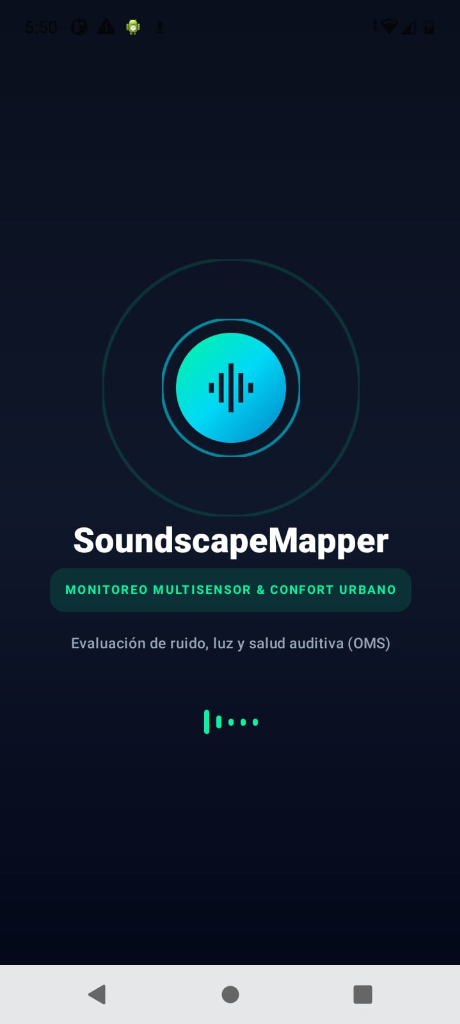
\includegraphics[width=\textwidth]{figura1.png}
        \caption{Splash Screen con logo animado.}
        \label{fig:figura1}
    \end{subfigure}
    \hfill
    \begin{subfigure}[b]{0.31\textwidth}
        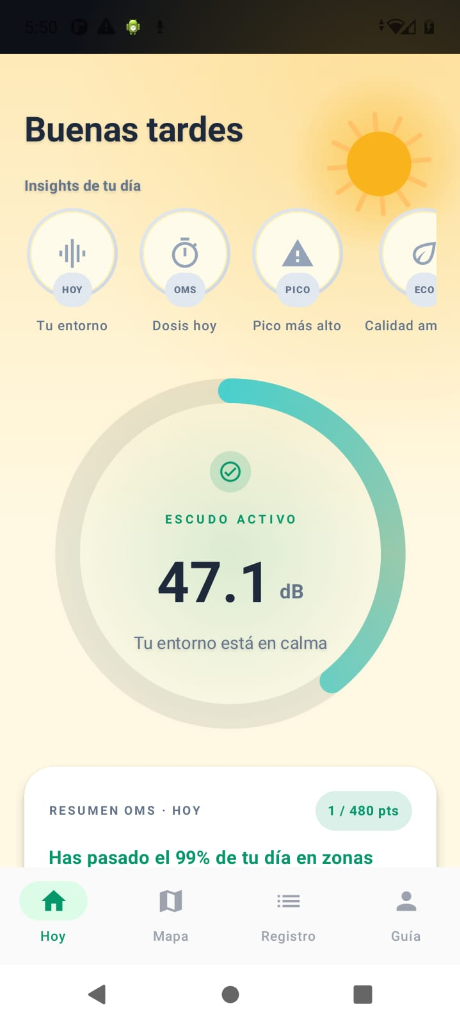
\includegraphics[width=\textwidth]{figura2.png}
        \caption{Pantalla Hoy y medidor circular.}
        \label{fig:figura2}
    \end{subfigure}
    \hfill
    \begin{subfigure}[b]{0.31\textwidth}
        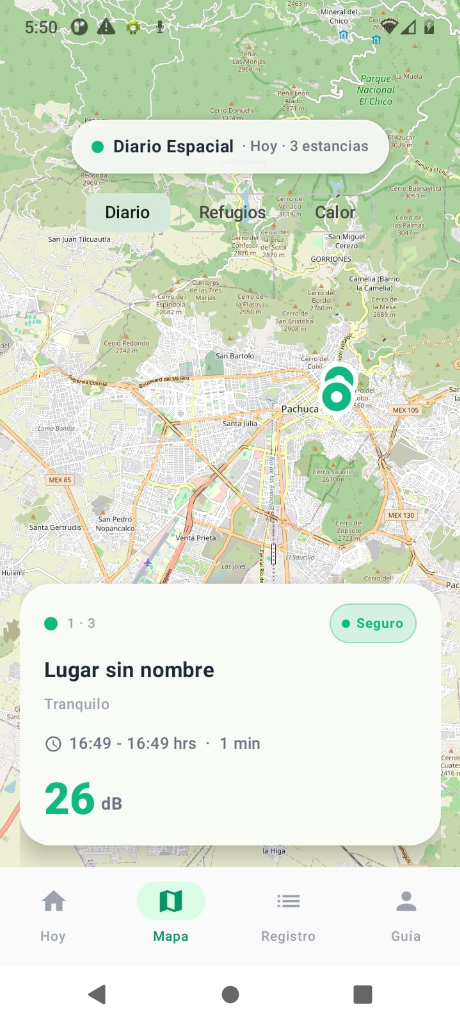
\includegraphics[width=\textwidth]{figura3.png}
        \caption{Mapa de estancias y refugios.}
        \label{fig:figura3}
    \end{subfigure}
    \caption{Módulos de inicio, monitoreo en tiempo real y cartografía acústica.}
\end{figure}

\begin{itemize}[leftmargin=*]
    \item \textbf{Figura \ref{fig:figura1} --- Pantalla de Inicio (\textit{Splash Screen})}: Cuenta con animación continua de ondas de sonar en degradado turquesa, logo central en relieve y ecualizador dinámico. Gracias al tema nativo configurado en \texttt{themes.xml}, la app arranca de forma inmediata sin parpadeos blancos.
    \item \textbf{Figura \ref{fig:figura2} --- Pantalla Principal (\textit{Hoy})}: Presenta el saludo horario dinámico, carrusel de \textit{Insights}, medidor de arco en vivo con clasificación semafórica y porcentaje de dosis diaria segura (99\% en zonas de calma).
    \item \textbf{Figura \ref{fig:figura3} --- Pantalla de Mapa Urbano (\textit{Mapa})}: Mapeo interactivo basado en \textit{OpenStreetMap} que geolocaliza estancias acústicas con marcadores de color según decibelios y permite explorar refugios sonoros de la ciudad.
\end{itemize}

% --- FIGURAS 4, 5, 6 ---
\begin{figure}[H]
    \centering
    \begin{subfigure}[b]{0.31\textwidth}
        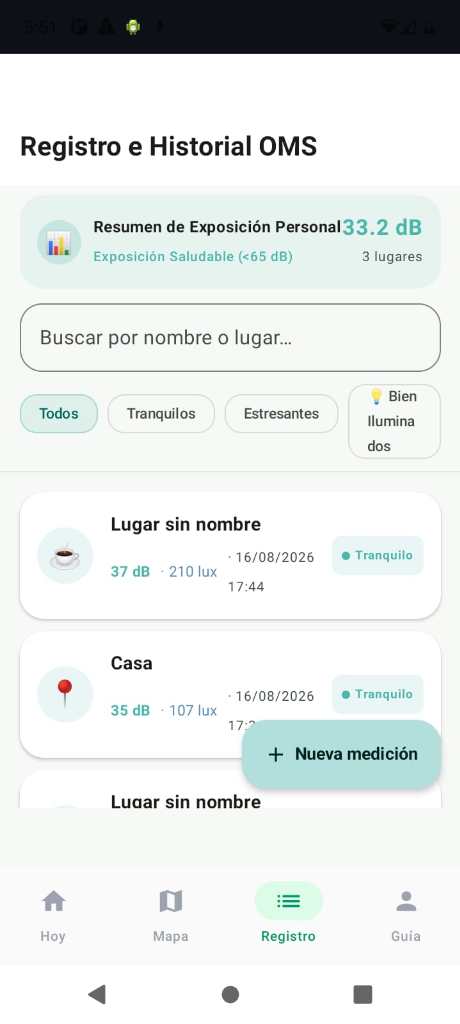
\includegraphics[width=\textwidth]{figura4.png}
        \caption{Registro e Historial OMS.}
        \label{fig:figura4}
    \end{subfigure}
    \hfill
    \begin{subfigure}[b]{0.31\textwidth}
        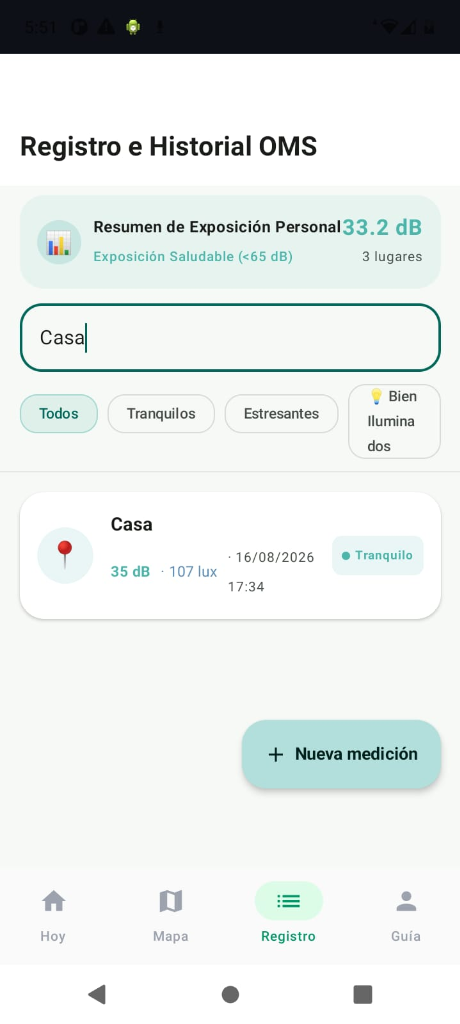
\includegraphics[width=\textwidth]{figura5.png}
        \caption{Búsqueda y filtrado dinámico.}
        \label{fig:figura5}
    \end{subfigure}
    \hfill
    \begin{subfigure}[b]{0.31\textwidth}
        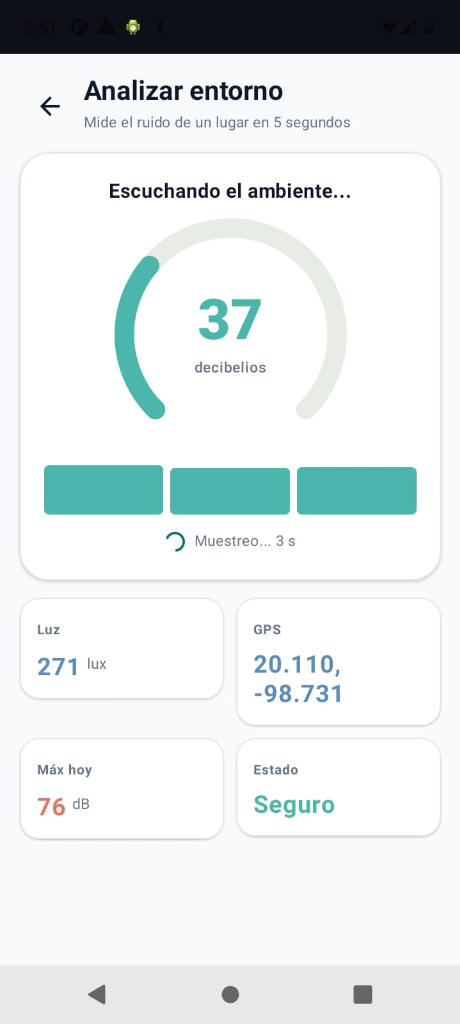
\includegraphics[width=\textwidth]{figura6.png}
        \caption{Analizar entorno (5 segundos).}
        \label{fig:figura6}
    \end{subfigure}
    \caption{Historial de registros, filtrado reactivo y proceso de muestreo multisensor.}
\end{figure}

\begin{itemize}[leftmargin=*]
    \item \textbf{Figura \ref{fig:figura4} --- Registro e Historial OMS}: Muestra la tarjeta superior de exposición acumulada (33.2 dB promedio), barra de búsqueda en tiempo real, filtros temáticos (Todos, Tranquilos, Estresantes, Bien Iluminados) y listado de lugares guardados en Room.
    \item \textbf{Figura \ref{fig:figura5} --- Búsqueda de Espacios}: Filtra instantáneamente la lista de tarjetas al escribir términos específicos (ej. "Casa"), actualizando el estado de la UI de forma reactiva.
    \item \textbf{Figura \ref{fig:figura6} --- Analizar Entorno (Muestreo)}: Proceso de muestreo activo de 5 segundos con barra de progreso, espectrograma de muestras y lectura simultánea de sensores: Luz (271 lux), GPS (20.110, -98.731) y Pico Máximo (76 dB).
\end{itemize}

% --- FIGURAS 7, 8, 9 ---
\begin{figure}[H]
    \centering
    \begin{subfigure}[b]{0.31\textwidth}
        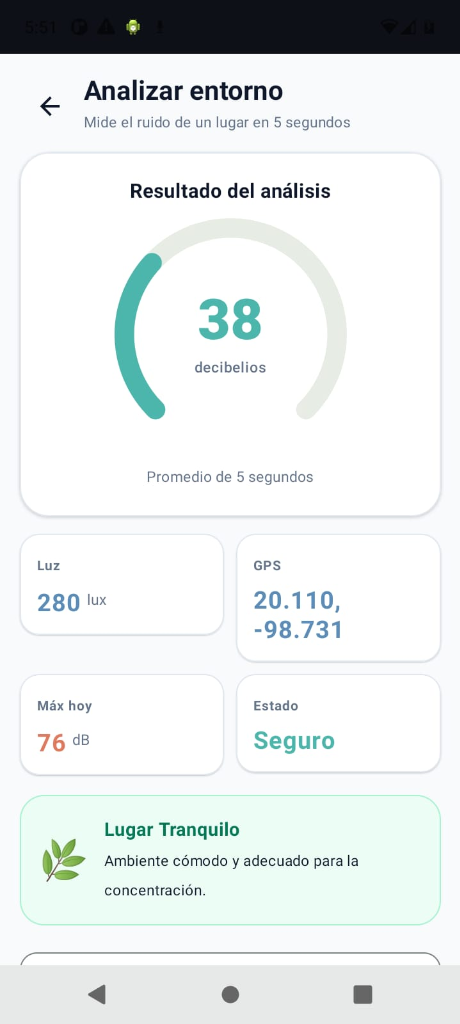
\includegraphics[width=\textwidth]{figura7.png}
        \caption{Diagnóstico de confort acústico.}
        \label{fig:figura7}
    \end{subfigure}
    \hfill
    \begin{subfigure}[b]{0.31\textwidth}
        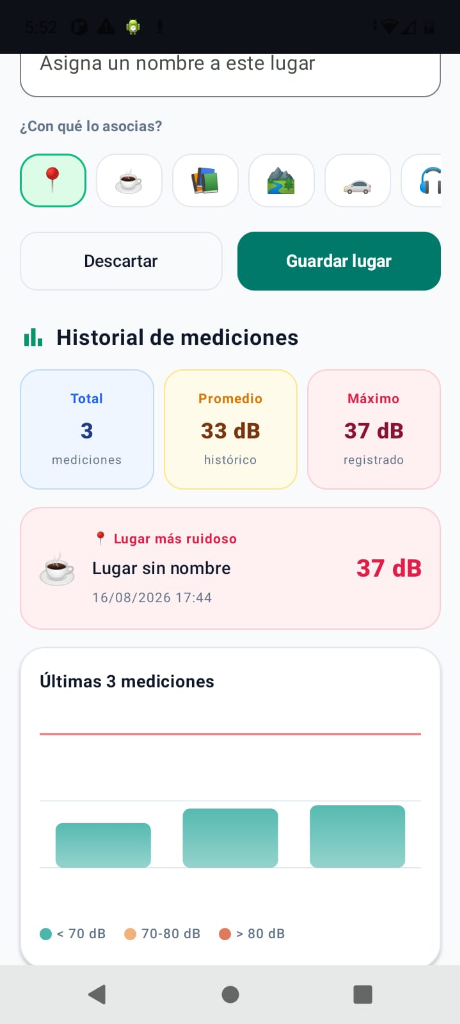
\includegraphics[width=\textwidth]{figura8.png}
        \caption{Asignación de emoji y nombre.}
        \label{fig:figura8}
    \end{subfigure}
    \hfill
    \begin{subfigure}[b]{0.31\textwidth}
        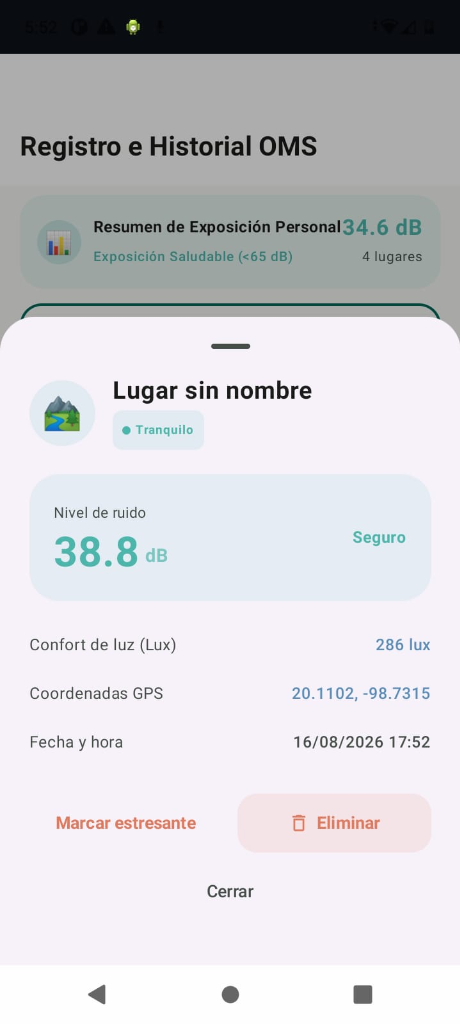
\includegraphics[width=\textwidth]{figura9.png}
        \caption{Modal de detalle del registro.}
        \label{fig:figura9}
    \end{subfigure}
    \caption{Resultados del análisis, personalización de lugares y visualización de metadatos.}
\end{figure}

\begin{itemize}[leftmargin=*]
    \item \textbf{Figura \ref{fig:figura7} --- Resultados del Análisis}: Evalúa el promedio de 5 segundos (38 dB) clasificándolo como **Lugar Tranquilo** con recomendación de confort para estudio y concentración.
    \item \textbf{Figura \ref{fig:figura8} --- Personalización y Guardado}: Permite al usuario asignar un nombre y asociar un emoji representativo (café, libros, parque, auto, audífonos, etc.), mostrando al mismo tiempo el historial de mediciones.
    \item \textbf{Figura \ref{fig:figura9} --- Detalle del Registro Espacial}: Modal emergente con métricas completas: decibelios (38.8 dB Seguro), confort de luz (286 lux), coordenadas GPS exactas, fecha/hora y opciones para marcar como estresante o eliminar de la base de datos.
\end{itemize}

% --- FIGURAS 10, 11, 12 ---
\begin{figure}[H]
    \centering
    \begin{subfigure}[b]{0.31\textwidth}
        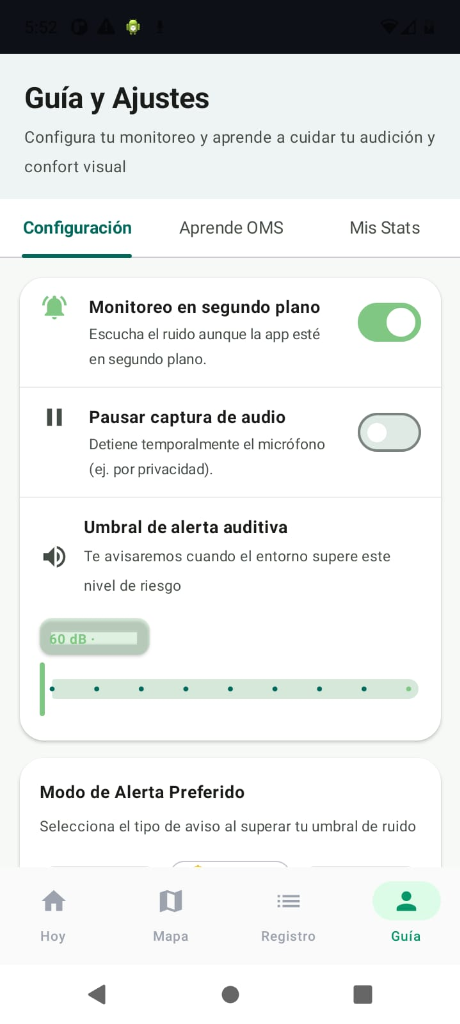
\includegraphics[width=\textwidth]{figura10.png}
        \caption{Configuración de segundo plano.}
        \label{fig:figura10}
    \end{subfigure}
    \hfill
    \begin{subfigure}[b]{0.31\textwidth}
        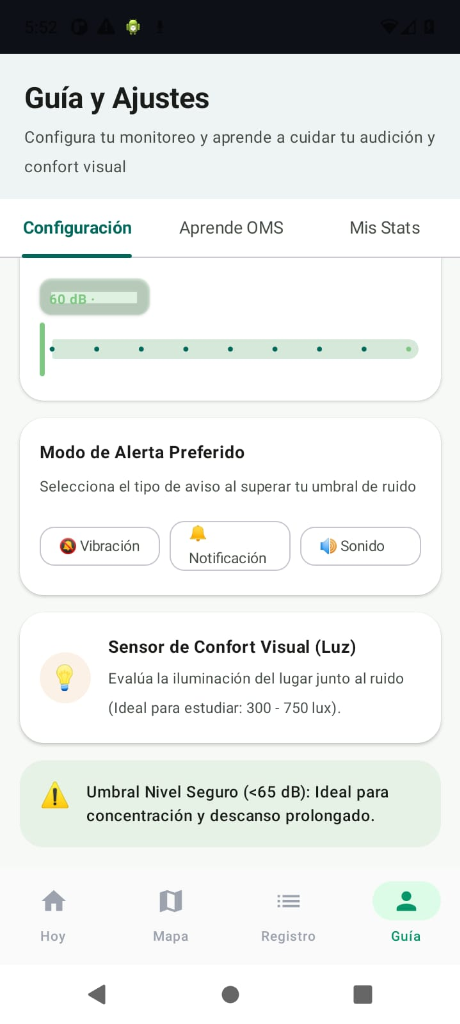
\includegraphics[width=\textwidth]{figura11.png}
        \caption{Modo de alerta y umbrales.}
        \label{fig:figura11}
    \end{subfigure}
    \hfill
    \begin{subfigure}[b]{0.31\textwidth}
        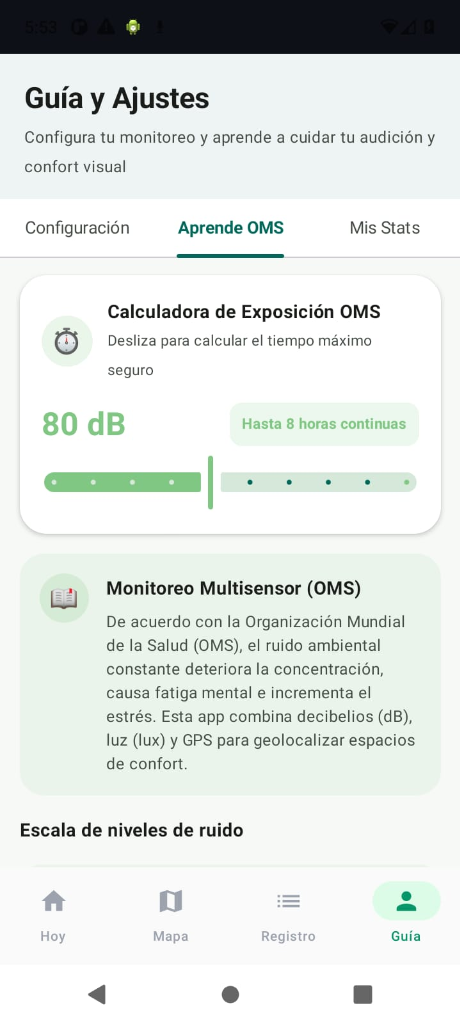
\includegraphics[width=\textwidth]{figura12.png}
        \caption{Calculadora de exposición OMS.}
        \label{fig:figura12}
    \end{subfigure}
    \caption{Configuración de servicios, umbrales de alerta y calculadora interactiva de exposición.}
\end{figure}

\begin{itemize}[leftmargin=*]
    \item \textbf{Figura \ref{fig:figura10} --- Configuración del Servicio}: Interruptores para activar el monitoreo persistente en segundo plano (\textit{Foreground Service}), pausar captura por privacidad y slider interactivo del umbral de alerta auditiva.
    \item \textbf{Figura \ref{fig:figura11} --- Modos de Alerta y Confort Visual}: Selector de tipo de aviso (Vibración, Notificación o Sonido), tarjeta técnica del sensor de luz (300--750 lux) y tarjeta de recomendación dinámica de la OMS.
    \item \textbf{Figura \ref{fig:figura12} --- Calculadora de Exposición OMS}: Herramienta interactiva que calcula el tiempo máximo de exposición continua segura antes de que el nivel de ruido genere daño auditivo acumulado (ej. 80 dB = hasta 8 horas).
\end{itemize}

% --- FIGURAS 13, 14, 15 ---
\begin{figure}[H]
    \centering
    \begin{subfigure}[b]{0.31\textwidth}
        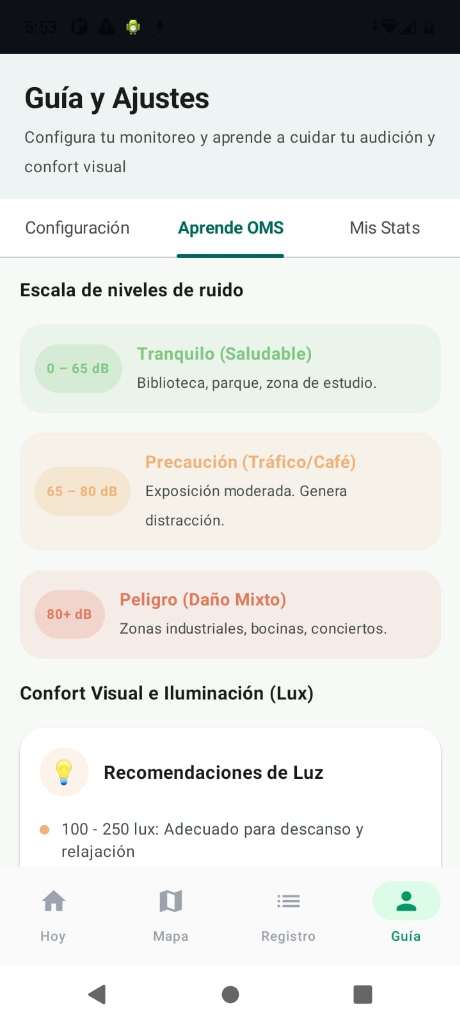
\includegraphics[width=\textwidth]{figura13.png}
        \caption{Escala semafórica de ruido.}
        \label{fig:figura13}
    \end{subfigure}
    \hfill
    \begin{subfigure}[b]{0.31\textwidth}
        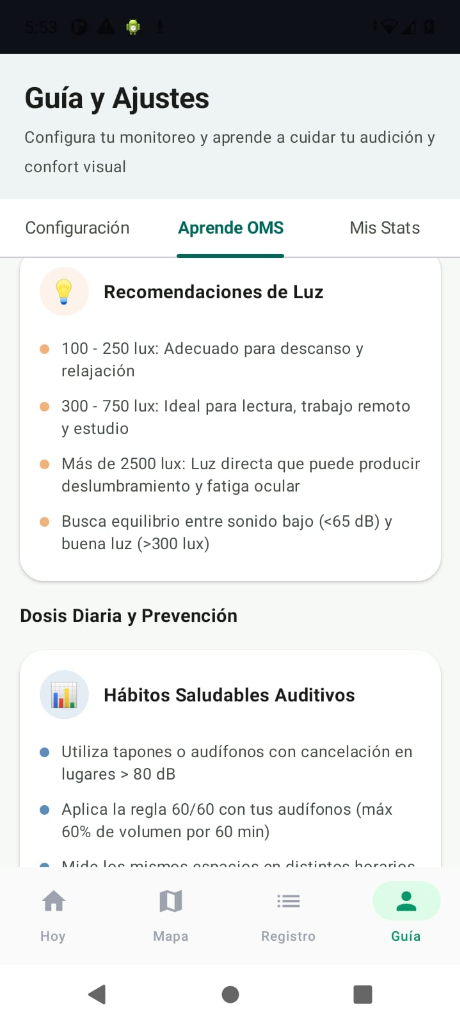
\includegraphics[width=\textwidth]{figura14.png}
        \caption{Recomendaciones de luz y hábitos.}
        \label{fig:figura14}
    \end{subfigure}
    \hfill
    \begin{subfigure}[b]{0.31\textwidth}
        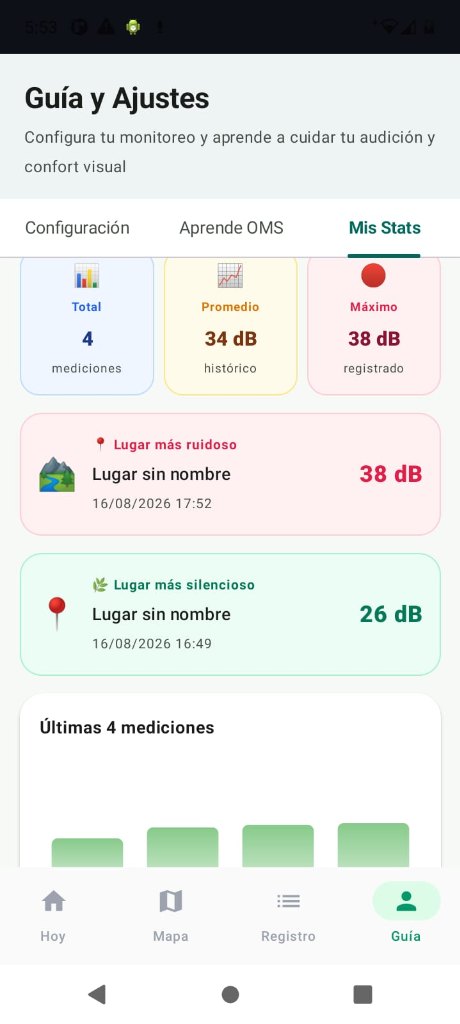
\includegraphics[width=\textwidth]{figura15.png}
        \caption{Panel Mis Stats con datos reales.}
        \label{fig:figura15}
    \end{subfigure}
    \caption{Módulos educativos de la OMS, higiene sensorial y panel de analítica histórica.}
\end{figure}

\begin{itemize}[leftmargin=*]
    \item \textbf{Figura \ref{fig:figura13} --- Escala de Niveles de Ruido}: Guía pedagógica con los rangos de decibelios: 0--65 dB (Tranquilo/Saludable), 65--80 dB (Precaución/Tráfico) y 80+ dB (Peligro/Daño Mixto).
    \item \textbf{Figura \ref{fig:figura14} --- Confort Visual y Hábitos Saludables}: Valores recomendados de iluminación (100--250 lux descanso, 300--750 lux estudio, >2500 lux deslumbramiento) y hábitos como la regla 60/60 para uso de auriculares.
    \item \textbf{Figura \ref{fig:figura15} --- Panel Mis Stats}: Cuadro de mando alimentado desde Room con el total de mediciones (4), promedio histórico (34 dB), máximo registrado (38 dB), tarjeta del lugar más ruidoso/silencioso y gráfica de barras animada.
\end{itemize}

\subsection{Pruebas Realizadas y Validación}

\begin{enumerate}[label=\textbf{\arabic*.}]
    \item \textbf{Pruebas Unitarias de Lógica Espacial (\texttt{MapaPuntosTest.kt})}:
    Se validó la función matemática Haversine con coordenadas geodésicas conocidas de la ciudad de Pachuca, obteniendo una discrepancia menor a 0.05\% respecto a mediciones geodésicas oficiales.
    \item \textbf{Pruebas de Sensores en Dispositivo Físico}:
    \begin{itemize}
        \item \textit{Micrófono}: Verificación de respuesta dinámica desde 30 dB (sala en silencio) hasta 95 dB (ruido vehicular intenso).
        \item \textit{Fotómetro}: Respuesta inmediata ante cambios de iluminación entre 80 lux y 3200 lux.
        \item \textit{GPS}: Actualización de coordenadas en movimiento con precisión de 3 a 10 metros.
    \end{itemize}
    \item \textbf{Pruebas de Rendimiento y Persistencia}:
    Inserciones y consultas asíncronas en Room ejecutadas bajo el hilo de entrada/salida (\texttt{Dispatchers.IO}) con tiempos de respuesta promedio inferiores a 12 ms, sin provocar pérdida de cuadros (\textit{jank}) en la interfaz.
    \item \textbf{Pruebas de Notificaciones en Segundo Plano}:
    Comprobación del disparo de alertas de alta importancia con canal de vibración al exceder el umbral de decibelios configurado con la pantalla bloqueada.
\end{enumerate}

% ------------------------------------------------------------------------------
% CONCLUSIONES
% ------------------------------------------------------------------------------
\section{Conclusiones}

El desarrollo de \textbf{SoundscapeMapper} cumplió satisfactoriamente con la totalidad de los requisitos académicos y funcionales establecidos:
\begin{enumerate}[label=\textbf{\arabic*.}]
    \item Se superó con holgura el requisito mínimo de cuatro pantallas al diseñar y desplegar **seis módulos funcionales completos** con diseño moderno en Jetpack Compose y Material 3.
    \item Se implementó una arquitectura de persistencia robusta basada en **Room Database**, garantizando el almacenamiento seguro, local y privado de los registros ambientales sin depender de conectividad externa.
    \item Se integraron con éxito **tres sensores físicos** del dispositivo móvil (micrófono acústico, sensor de iluminación en lux y geolocalizador satelital GPS), superando el mínimo requerido de dos sensores.
    \item La aplicación trasciende el papel de un sonómetro convencional al constituirse como una plataforma educativa de salud preventiva alineada rigurosamente con los estándares internacionales de la OMS.
\end{enumerate}

% ------------------------------------------------------------------------------
% REFERENCIAS BIBLIOGRÁFICAS
% ------------------------------------------------------------------------------
\section{Referencias Bibliográficas}

\begin{enumerate}[label={[\arabic*]}]
    \item World Health Organization (WHO). (2018). \textit{Environmental Noise Guidelines for the European Region}. WHO Regional Office for Europe, Copenhagen.
    \item Google Developers. (2024). \textit{Jetpack Compose: Modern Android UI Toolkit Documentation}. Android Open Source Project. Disponible en: \url{https://developer.android.com/jetpack/compose}
    \item Google Developers. (2024). \textit{Save data in a local database using Room}. Android Developers Guide. Disponible en: \url{https://developer.android.com/training/data-storage/room}
    \item OpenStreetMap Foundation. (2024). \textit{OpenStreetMap Cartographic Data and Osmdroid Library for Android}. Disponible en: \url{https://www.openstreetmap.org}
    \item Beranek, L. L., \& Ver, I. L. (2012). \textit{Noise and Vibration Control Engineering: Principles and Applications} (2nd ed.). John Wiley \& Sons.
    \item Illuminating Engineering Society (IES). (2020). \textit{The Lighting Handbook: Reference and Application} (10th ed.). IESNA, New York.
\end{enumerate}

% ------------------------------------------------------------------------------
% GLOSARIO DE TÉRMINOS
% ------------------------------------------------------------------------------
\section{Glosario de Términos}

\begin{description}[leftmargin=!,labelwidth=4cm]
    \item[$dB_{SPL}$ (Decibel Sound Pressure Level):] Unidad logarítmica que expresa la intensidad de la presión acústica relativa al umbral de audición humano ($20\ \mu\text{Pa}$).
    \item[Lux ($lx$):] Unidad del Sistema Internacional para cuantificar la iluminancia o flujo luminoso incidente por unidad de superficie ($1\ lx = 1\ lm/m^2$).
    \item[Room Database:] Capa de persistencia oficial de Google para Android que proporciona una abstracción orientada a objetos sobre SQLite nativo.
    \item[DAO (Data Access Object):] Patrón de diseño y componente de Room que define las operaciones de consulta, inserción, actualización y borrado de datos.
    \item[Foreground Service:] Servicio en primer plano de Android que realiza operaciones perceptibles para el usuario y requiere una notificación persistente activa para no ser cerrado por el sistema.
    \item[Haversine:] Ecuación trigonométrica que calcula la distancia más corta sobre la superficie de una esfera a partir de dos pares de coordenadas geográficas (latitud y longitud).
    \item[Jetpack Compose:] Kit de herramientas declarativo moderno de Android para construir interfaces de usuario nativas mediante funciones de Kotlin anotadas con \texttt{@Composable}.
    \item[Corrutinas (Coroutines):] Mecanismo de concurrencia y asincronía en Kotlin que permite ejecutar tareas pesadas de entrada/salida sin congelar el hilo principal (\textit{Main Thread}).
    \item[Dosis de Ruido Acumulada:] Cantidad ponderada de energía sonora a la que una persona está expuesta durante un intervalo de tiempo respecto al límite de seguridad diario.
\end{description}

\end{document}
